\documentclass[12pt,a4paper]{article}
\usepackage[left=3cm,right=2.5cm,top=2.5cm,bottom=2.5cm,headheight=15pt]{geometry}
\usepackage[T1]{fontenc}
\usepackage{tgtermes}
\usepackage[utf8,nocaptions]{vietnam}
\usepackage{setspace}
\usepackage{fancyhdr}
\usepackage{titlesec}
\usepackage{indentfirst}
\usepackage{placeins}
\usepackage{needspace}
\usepackage{enumitem}
\usepackage{fancyvrb}
\RecustomVerbatimEnvironment{verbatim}{Verbatim}{fontsize=\small}
\setlist{topsep=4pt,itemsep=3pt,parsep=0pt}
\raggedbottom
\widowpenalty=10000
\clubpenalty=10000
\setcounter{topnumber}{3}
\setcounter{bottomnumber}{2}
\setcounter{totalnumber}{5}
\renewcommand{\topfraction}{0.9}
\renewcommand{\bottomfraction}{0.8}
\renewcommand{\textfraction}{0.1}
\renewcommand{\floatpagefraction}{0.75}
\setlength{\textfloatsep}{12pt plus 2pt minus 2pt}
\setlength{\intextsep}{10pt plus 2pt minus 2pt}
\setlength{\floatsep}{10pt plus 2pt minus 2pt}
\setstretch{1.10}
\setlength{\parindent}{1cm}
\setlength{\parskip}{3pt}
\setlength{\emergencystretch}{2em}
\setcounter{tocdepth}{2}
\setcounter{secnumdepth}{3}
\renewcommand{\contentsname}{TABLE OF CONTENTS}
\renewcommand{\listfigurename}{LIST OF FIGURES}
\renewcommand{\listtablename}{LIST OF TABLES}
\titleformat{\section}{\normalfont\Large\bfseries}{\thesection.}{0.5em}{}
\titleformat{\subsection}{\normalfont\large\bfseries}{\thesubsection.}{0.5em}{}
\titleformat{\subsubsection}{\normalfont\normalsize\bfseries}{\thesubsubsection.}{0.5em}{}
\titlespacing*{\section}{0pt}{16pt}{10pt}
\titlespacing*{\subsection}{0pt}{12pt}{7pt}
\titlespacing*{\subsubsection}{0pt}{9pt}{5pt}
\fancypagestyle{report}{
\fancyhf{}
\fancyhead[L]{\small Trustworthy AI -- Course Project}
\fancyhead[R]{\small\nouppercase{\leftmark}}
\fancyfoot[C]{\thepage}
\renewcommand{\headrulewidth}{0.4pt}}
\renewcommand{\sectionmark}[1]{\markboth{\thesection.\ #1}{}}
\fancypagestyle{plain}{\fancyhf{}\fancyfoot[C]{\thepage}\renewcommand{\headrulewidth}{0pt}}
\usepackage{amsmath,amssymb,amsthm}
\usepackage{booktabs}
\usepackage{graphicx}
\usepackage{hyperref}
\usepackage[numbers,sort&compress]{natbib}
\usepackage{caption}
\usepackage{subcaption}
\captionsetup{font=small,skip=6pt}
\usepackage{float}
\usepackage{xcolor}
\hypersetup{hidelinks}

\title{Spurious Correlations and Invariant Learning:\\ ERM vs IRM vs REx on Colored-MNIST}
\author{Trustworthy AI --- Course Project (Reliability Pillar)}
\date{October 2026}

\begin{document}

% ---------------- Cover page (HUST standard, borrowed) ----------------
\begin{titlepage}
\setstretch{1}
\setlength{\parskip}{0pt}
\centering
{\fontsize{15}{18}\selectfont\bfseries HANOI UNIVERSITY OF SCIENCE AND TECHNOLOGY\par}
\vspace{4mm}
{\fontsize{12}{15}\selectfont\bfseries SCHOOL OF INFORMATION AND COMMUNICATION TECHNOLOGY\par}
\vspace{12mm}
{\fontsize{15.5}{19}\selectfont\bfseries COURSE PROJECT REPORT\par}
\vspace{4mm}
{\normalsize Course: Trustworthy AI\par}
\vspace{14mm}
\rule{0.86\linewidth}{0.8pt}\par
\vspace{8mm}
{\fontsize{19.5}{25}\selectfont\bfseries \shortstack{SPURIOUS CORRELATIONS AND\\INVARIANT LEARNING}\par}
\vspace{3mm}
{\large\bfseries ERM vs IRM vs REx on Colored-MNIST\par}
\vspace{8mm}
\rule{0.86\linewidth}{0.5pt}\par
\vspace{12mm}
% SUPERVISOR: replace the dotted line with the name and academic title.
{\textbf{Supervisor:}\quad Dr.\ Nguyễn Đức Anh\par}
\vspace{10mm}
{\bfseries TEAM MEMBERS\par}
\vspace{3mm}
% ============================================================
% TEAM INFORMATION — enter the student IDs and full names below.
% Member 1: student ID / full name (add Team Leader if applicable).
% Member 2: student ID / full name.
% Member 3: student ID / full name.
% Add or remove rows to match the actual team.
% ============================================================
\renewcommand{\arraystretch}{1.45}
\begin{tabular}{ll}
\toprule
\textbf{Student ID} & \textbf{Full Name} \\
\midrule
20261081M & Nguyễn Hoàng Nam \\
20261077M & Ngô Ngọc Sâm \\
20261058M & Nguyễn Hữu Tâm \\
202610
\bottomrule
\end{tabular}
\vfill
{\normalsize Hanoi, October 2026\par}
\end{titlepage}

\pagenumbering{roman}
\pagestyle{plain}
\section*{ABSTRACT}
\noindent
Machine learning models can perform well on in-distribution data but fail under 
distribution shift when they rely on spurious correlations. This report studies 
this problem using Colored-MNIST, where digit shape is the stable signal and color 
is spuriously correlated with the label during training but largely reversed at test 
time. We compare ERM, IRMv1, and V-REx under the same training and evaluation 
pipeline using multiple random seeds and train-domain validation as the primary 
model-selection protocol. Additional experiments examine the effects of penalty 
strength, backbone architecture, number of environments, additional spurious features, 
sample size, and dataset choice. The results show that ERM performs well on the training 
environments but degrades substantially under the OOD setting. IRMv1 is strongly 
affected by model selection and also shows considerable variation across random seeds. 
V-REx provides more stable behavior across the tested penalty settings. 
The ablation experiments further show that invariant learning becomes more 
difficult when the number of environments is reduced or additional spurious 
features are introduced. Diagnostic analyses using calibration, Integrated Gradients, 
and linear probes show that reduced reliance on color does not necessarily mean 
that color information is removed from the learned representation. 
Overall, the results highlight the importance of model selection, repeated runs, 
and diagnostic analysis when evaluating OOD generalization under spurious correlations.

\medskip
\noindent\textbf{Keywords:} spurious correlation, invariant learning, IRM, 
V-REx, OOD generalization, model selection, trustworthy AI.
\clearpage

\begingroup
\small
\tableofcontents
\endgroup
\clearpage
\listoffigures
\clearpage
\listoftables

% ============================================================
% ============================================================
% PART 1 — INTRODUCTION
% ============================================================
\clearpage
\pagenumbering{arabic}
\pagestyle{report}
\section{Introduction}\label{sec:intro}

Some machine learning models achieve high accuracy on in-distribution data; 
however, they may fail under distribution shift, resulting in poor 
performance in practical applications. One reason for this problem is that some 
features are correlated with the target label in the training data, but this 
correlation does not hold in real-world settings. 
This is called a \emph{spurious correlation}. A common example of this phenomenon 
is the cow-camel classification problem, where cows are predominantly observed 
on grassy backgrounds while camels are associated with sandy backgrounds in the 
training data. As a result, a classifier may learn to rely on the background 
rather than the characteristics of the animal itself, leading to poor performance 
when this correlation changes at test time \citep{nagarajan2021understanding}.

To study this problem, we set up a controlled environment using \textbf{Colored-MNIST}
\citep{arjovsky2019irm}, where digit shape serves as the stable signal, while
color is spuriously correlated with the label during training and anti-correlated
at test time. This setting provides a simple way to observe how models behave when
a spurious correlation is present and how different training objectives respond to
changes in the data distribution. Based on this setup, the report focuses on the
following research questions:

\begin{itemize}
\item \textbf{RQ1 (reproduce):} Does ERM rely on color and experience a drop in OOD performance, 
and how do invariant learning objectives behave under the same setting?
\item \textbf{RQ2 (break):} Under what conditions does invariant learning become less 
effective, considering penalty strength, backbone capacity, number of environments, 
a second spurious feature, sample size, and dataset choice?
\item \textbf{RQ3 (diagnose):} Which diagnostics can help indicate whether a model relies 
less on color, including calibration, attribution methods, and representation probes?
\end{itemize}

The report includes three main parts:
\begin{enumerate}
\item We evaluate ERM, IRMv1, and V-REx across three random seeds and report the mean$\pm$std 
results under two model-selection protocols: train-domain validation and OOD oracle 
\citep{domainbed2021}.
\item We conduct 18 ablation settings covering the IRM-$\lambda$ sweep, REx-$\beta$ 
sweep, MLP and CNN backbones, single-environment training, a second spurious patch, 
small-$n$ settings, and transfer to Colored-FashionMNIST\@
\item We examine model behavior using reliability analysis, Integrated Gradients, 
and linear probes, with particular attention to the Reliability and Explainability 
aspects of trustworthy AI\@
\end{enumerate}
% ============================================================
% ============================================================
% PART 2 — RELATED WORK
% ============================================================
\clearpage
\section{Related work}\label{sec:related}

\subsection{Invariant Risk Minimization (IRM)}
\citet{arjovsky2019irm} introduce Invariant Risk Minimization (IRM), which aims to learn a 
representation $\Phi$ such that the same classifier $w$ performs well across all training environments. 
In practice, the commonly used IRMv1 objective adds a gradient-based penalty to 
encourage this invariance (see \S\ref{sec:problem}). Later studies show that IRMv1 
can be sensitive to the random seed and the penalty weight $\lambda$. 
Several extensions have therefore been proposed, including game-based 
optimization \citep{irmgames2020}, gradient-variance regularization such as 
Fishr \citep{rame2022fishr}, and sparse variants of IRM \citep{zhou2022sparseirm}.

\subsection{Risk Extrapolation (REx) and Group DRO}
V-REx \citep{krueger2021rex} encourages similar risks across training environments 
by penalizing the variance of environment-wise risks. This provides a simpler 
alternative to the IRMv1 penalty. Group DRO \citep{sagawa2020dro} takes a 
different approach by minimizing the loss of the worst-performing environment. 
In this report, a simplified Group DRO objective is included as an additional 
reference method.

\subsection{Limitations of invariant learning}
Previous work also studies cases where invariant learning may not work as expected. 
\citet{rosenfeld2021risks} show that IRM requires enough training environments 
relative to the number of spurious features, and that learning from a single 
environment is not sufficient in their setting.\ \citet{zhou2022sparseirm} further
show that over-parameterized models can make invariant learning more difficult. 
These results motivate several of the stress tests used in our experiments.

\subsection{Model selection and diagnostic methods}
Model selection is also important when evaluating OOD generalization. 
DomainBed \citep{domainbed2021} shows that reported performance can depend 
strongly on how models are selected, especially when comparing train-domain 
validation with OOD-based selection. In addition, DFR \citep{kirichenko2022dfr} 
and JTT \citep{liu2021jtt} suggest that useful features may already be 
present in the learned representation even when the final classifier 
does not use them effectively. This motivates the use of linear probes 
in our analysis. For explainability, we use Integrated Gradients 
\citep{sundararajan2017ig} as the main attribution method, while vanilla 
saliency is kept only as a simple baseline because of known 
limitations \citep{adebayo2018sanity}.
% ============================================================
% ============================================================
% PART 3 — PROBLEM FORMULATION AND METHODS
% ============================================================
\clearpage
\section[Problem formulation and methods]{Problem formulation and methods}\markboth{3. Problem formulation and methods}{}
\label{sec:problem}

\subsection{Structural causal model}
Let $D \in \{0,\dots,9\}$ denote the original MNIST digit. We first define the binary
label $\tilde{Y} = \mathbf{1}[D \ge 5]$, which separates digits $0$--$4$ from digits
$5$--$9$. To introduce label noise, the observed label is generated as
$Y = \mathrm{flip}(\tilde{Y};0.25)$, meaning that the binary label is flipped with
probability $0.25$.

The color variable $C$ is then generated from the observed label as
$C = \mathrm{flip}(Y;p_e)$, where $p_e$ depends on the environment $e$.
The final image $X \in \mathbb{R}^{3 \times 28 \times 28}$ contains the original
digit shape rendered in red when $C=0$ and in green when $C=1$.

This construction separates two sources of information. The digit shape is determined
by $D$ and remains unchanged across environments, so it acts as the stable signal.
In contrast, the relationship between color $C$ and the observed label $Y$ depends on
$p_e$, so color acts as the spurious signal. By changing $p_e$ between training and
test environments, we can directly study whether a model relies on the stable signal
or on the easier but environment-dependent color signal.

\subsection{Input}
The input to the model is a colored digit image
$x \in \mathbb{R}^{3 \times 28 \times 28}$.
Each input contains both the original digit shape and the assigned color.
The shape carries information about the underlying digit $D$, while the color is
introduced according to the environment-specific variable $C$.

Because both signals are available in the same image, the model can potentially solve
the task using either of them. However, only the digit shape remains reliable when the
data distribution changes across environments.

\subsection{Output}
The task is binary classification. Given an input image $x$, the model estimates
the probability
\[
P(Y=1 \mid X=x),
\]
and produces a prediction $\hat{y} \in \{0,1\}$.

The target label is derived from the original digit group:
digits $0$--$4$ correspond to $\tilde{Y}=0$, while digits $5$--$9$ correspond to
$\tilde{Y}=1$. The observed label $Y$ is obtained after applying the $25\%$ label
noise described above. Therefore, even a classifier that perfectly recovers the
digit group cannot achieve perfect accuracy with respect to $Y$.

\subsection{Environments}
We use two training environments and one OOD test environment:
\[
e_1: p_e=0.1, \qquad
e_2: p_e=0.2, \qquad
e_{\mathrm{te}}: p_e=0.9.
\]

The parameter $p_e$ controls the probability that the color is flipped relative to
the observed label. When $p_e$ is small, color is strongly correlated with the label.
Therefore, in the two training environments, color provides an easy predictive signal.
In the OOD test environment, however, $p_e=0.9$, so this relationship is almost
reversed.

This shift creates the main difficulty of the task. A classifier that mainly uses
color can perform well on the training distribution but fail when evaluated on the
OOD environment. In contrast, a classifier that relies on digit shape is unaffected
by the change in color correlation.

Under this construction, a color-only rule achieves approximately $0.85$ ID accuracy
but only around $0.10$ OOD accuracy. A shape-only oracle achieves approximately $0.75$
accuracy across all environments, with this upper bound caused by the $25\%$ label noise.

\subsection{Learning objectives}
For each environment $e$, let

\[
R^e(\theta)
=
\mathbb{E}_{(x,y)\sim P_e}
\left[
\ell(f_\theta(x),y)
\right],
\]

where $\ell$ denotes the binary cross-entropy loss and $R^e(\theta)$ is the risk of
model $f_\theta$ in environment $e$. The methods considered in this report use the
same environment-specific risks but optimize them using different objectives.

\subsubsection{Empirical Risk Minimization (ERM)}
ERM minimizes the average risk across all training environments:

\[
\min_\theta
\frac{1}{E}
\sum_e R^e(\theta).
\]

ERM does not explicitly distinguish between stable and spurious signals. Therefore,
if color provides an easier predictive signal during training, the model may rely on
color even when this relationship does not remain valid in the OOD environment.

\subsubsection{Invariant Risk Minimization (IRMv1)}
IRM aims to learn a representation for which the same classifier remains suitable
across different training environments. In practice, IRMv1 introduces a
gradient-based penalty:

\[
\min_\Phi
\sum_e R^e(w \circ \Phi)
+
\lambda
\sum_e
\left\|
\nabla_{w=1} R^e(w \cdot \Phi)
\right\|^2.
\]

The penalty encourages the learned representation to support a shared classifier
across environments. In our experiments, the penalty is activated after an annealing
period of 190 optimization steps, so $\lambda=0$ before step 190.

\subsubsection{Variance Risk Extrapolation (V-REx)}
V-REx encourages the model to achieve similar risks across training environments.
Its objective is defined as

\[
\min_\theta
\mathrm{mean}_e\left(R^e\right)
+
\beta
\cdot
\mathrm{Var}_e\left(R^e\right),
\]

where $\beta$ controls the strength of the variance penalty. A larger value of
$\beta$ places more emphasis on reducing differences in risk between environments.

\subsubsection{GroupDRO-lite}
GroupDRO-lite focuses on the environment with the highest risk and minimizes the
worst-environment loss:

\[
\min_\theta
\max_e R^e(\theta).
\]

Unlike ERM, which optimizes the average risk, this objective gives more attention to
the environment in which the model currently performs worst. In this report,
GroupDRO-lite is included as an additional reference objective rather than a main
method of analysis.

For IRMv1, we use the standard dummy-classifier formulation with $w=1.0$ to compute
the gradient penalty. Evaluation metrics, dataset sizes, and the model-selection
protocol used throughout the experiments are described in
\S\ref{subsec:protocol}.
% ============================================================
\begingroup
\setstretch{1.05}
\subsection{Implementation and optimization}
\label{sec:method}

\subsubsection{Pipeline}
The implementation follows a simple
\texttt{data}$\rightarrow$\texttt{train}$\rightarrow$\texttt{eval}$\rightarrow$\texttt{viz}
pipeline.

The data module, \texttt{src/cmnist/data.py}, constructs the Colored-MNIST datasets
following the protocol introduced by \citet{arjovsky2019irm}. It also supports
Colored-FashionMNIST and an optional $3\times3$ spurious patch used in several
failure-case experiments. Each generated sample is assigned to a predefined
environment according to the corresponding color-flip probability.

The training stage receives these environment-specific datasets together with a model
architecture and a learning objective. The same pipeline is used across all experiments
so that differences in results mainly come from the objective, model architecture,
or experimental setting rather than from changes in the training procedure.

\subsubsection{Models and optimization}
Two backbone architectures are used. The first is a multilayer perceptron (MLP) with
two hidden layers of 256 units each. The second is a small convolutional neural network
(CNN), which provides a higher-capacity image-specific backbone for comparison.

The learning objectives are implemented in \texttt{losses.py} and include ERM, IRMv1,
V-REx, and GroupDRO-lite. Training is handled by \texttt{train.py} using the Adam
optimizer with a learning rate of $10^{-3}$, a batch size of 2048, and 2000
optimization steps for the main experiments.

For objectives that use a penalty term, the penalty is activated only after an
annealing period of 190 steps. Before this threshold, the penalty weight is set to
zero. Therefore, IRMv1 and V-REx initially behave like ERM and only begin enforcing
their additional constraints after the annealing stage.

During training, the pipeline records checkpoints according to both ID validation
performance and OOD performance. These checkpoints are later used to compare the
effect of different model-selection protocols.

\subsubsection{Evaluation}
The evaluation module, \texttt{eval.py}, measures model performance separately for
each environment. The reported metrics include per-environment accuracy, worst-group
accuracy, the performance gap between environments, and Expected Calibration Error
(ECE).

These metrics are intended to capture different aspects of model behavior. Accuracy
measures predictive performance, worst-group accuracy reflects the weakest environment,
the environment gap indicates how much performance changes under distribution shift,
and ECE provides information about calibration.

Additional diagnostic outputs, including attribution maps and linear-probe results,
are produced for the analysis in RQ3. Visualization utilities are separated from the
training and evaluation code so that the same trained checkpoints can be reused for
different diagnostic analyses.

\subsubsection{Experiment budget}
To manage the experimental workload, we use three execution modes.

\begin{itemize}
    \item \texttt{fast}: 500 training steps and one random seed, used mainly to verify
    that the full pipeline runs correctly.
    
    \item \texttt{base}: 2000 training steps for ERM, IRMv1, and V-REx across three
    random seeds. This configuration is used for the main comparison in RQ1.
    
    \item \texttt{heavy}: extended experiments including penalty sweeps, backbone
    comparisons, failure-case variants, and transfer to Colored-Fashion\-MNIST.
    This configuration contains 54 runs in total.
\end{itemize}

All main experiments use random seeds $\{0,1,2\}$. Deterministic cuDNN settings are
enabled to reduce variation caused by non-deterministic GPU operations. The full
experimental suite requires approximately three hours of GPU time on a Colab T4
with 16\,GB of memory.

% ============================================================
% ============================================================
\endgroup
% PART 4 — EXPERIMENTAL SETUP
% ============================================================
\clearpage
\section{Experimental setup}\label{sec:experiments}

\subsection{Purpose of evaluation}\label{subsec:purpose}

The experimental evaluation is designed around the three research questions introduced
in \S\ref{sec:intro}. For \textbf{RQ1 (reproduce)}, we examine how ERM behaves under
distribution shift and compare it with invariant learning objectives under the same
model-selection protocol. For \textbf{RQ2 (break)}, we study how the behavior of
invariant learning changes when varying the penalty strength, backbone capacity, number
of environments, number of spurious features, sample size, and dataset. For
\textbf{RQ3 (diagnose)}, we use calibration, attribution methods, and representation
probes to investigate whether the model reduces its reliance on the spurious feature.

Section~\ref{sec:results} presents the results according to these three research questions.

\subsection{Evaluation protocol}
\label{subsec:protocol}

\subsubsection{Data}
All experiments follow the Colored-MNIST construction described in
\S\ref{sec:problem}. The original MNIST training set is divided into two disjoint
training environments, each containing approximately 30,000 images. The first
environment uses $p_e=0.1$, while the second uses $p_e=0.2$. The full MNIST test set,
containing 10,000 images, is used as the OOD test environment with $p_e=0.9$, where
the correlation between color and label is largely reversed.

For the small-$n$ experiments, each training environment is reduced to 6,250 samples
to examine the effect of limited training data. For the dataset-transfer experiments,
the same environment-generation procedure is applied to FashionMNIST, allowing us to
observe whether the behavior found on Colored-MNIST also appears on a different image
dataset.

\subsubsection{Metrics}
We report several performance metrics. The average ID accuracy across the two
training environments is

\[
\text{ID-avg}
=
\frac{\mathrm{Acc}_{e_1}+\mathrm{Acc}_{e_2}}{2}.
\]

OOD accuracy is the classification accuracy on the held-out test environment,

\[
\text{OOD accuracy}
=
\mathrm{Acc}_{e_{\mathrm{te}}}.
\]

To measure the change in performance under distribution shift, we also report the
OOD gap:

\[
\text{OOD gap}
=
\text{ID-avg} - \text{OOD accuracy}.
\]

A larger gap indicates a larger reduction in accuracy when moving from the training
environments to the OOD environment.

To examine performance across combinations of label and color, the test samples are
divided into groups $g=(y,c)\in\{0,1\}^2$. We report the worst-group accuracy as

\[
\text{Worst-group accuracy}
=
\min_g \mathrm{Acc}_g.
\]

This metric indicates whether good average performance hides particularly poor
performance on one label--color subgroup. Finally, model calibration is evaluated
using Expected Calibration Error (ECE) with 15 confidence bins.

\subsubsection{Model selection}
The primary model-selection protocol is \textbf{train-domain validation}, where the
checkpoint with the highest ID-avg validation accuracy is selected without using
information from the OOD test environment. This protocol is used for the main
experimental results.

For comparison, we also report an \textbf{OOD oracle} result, where the checkpoint is
selected directly according to OOD test accuracy. Since this protocol uses information
from the test environment, it is not used as the primary evaluation setting; instead,
it provides a reference for examining the effect of model-selection strategy.

Unless otherwise stated, all reported results are presented as mean$\pm$standard
deviation over three random seeds.

% ============================================================
% PART 5 — RESULTS AND DISCUSSION
% ============================================================
\clearpage
\section{Results and discussion}\label{sec:results}

\subsection{Main comparison (RQ1)}

Table~\ref{tab:main} and Fig.~\ref{fig:accbar} summarize the main comparison under
the train-domain validation protocol. ERM achieves very high accuracy on the training
environments but shows a substantial decrease in OOD accuracy. IRMv1 shows a similar
drop, together with noticeably larger variation across random seeds. In contrast,
V-REx achieves higher average OOD accuracy and lower seed variance than ERM and IRMv1
under this evaluation setting.

\begin{table}[!htbp]
\centering
\small
\setlength{\tabcolsep}{4pt}
\caption{Main OOD comparison under train-domain validation
(mean$\pm$std over 3 seeds).}\label{tab:main}
\begin{tabular}{lccccc}
\toprule
Method & Train (ID avg) & Test (OOD) & OOD gap & Worst group & ECE \\
\midrule
ERM & 0.994 & 0.315 $\pm$ 0.010 & 0.679 & 0.243 $\pm$ 0.010 & 0.017 \\
IRMv1 & 0.801 & 0.243 $\pm$ 0.172 & 0.558 & 0.010 $\pm$ 0.009 & 0.309 \\
V-REx & 0.806 & 0.424 $\pm$ 0.014 & 0.382 & 0.339 $\pm$ 0.035 & 0.058

\\
\bottomrule
\end{tabular}
\end{table}

\begin{figure}[!htbp]
\centering
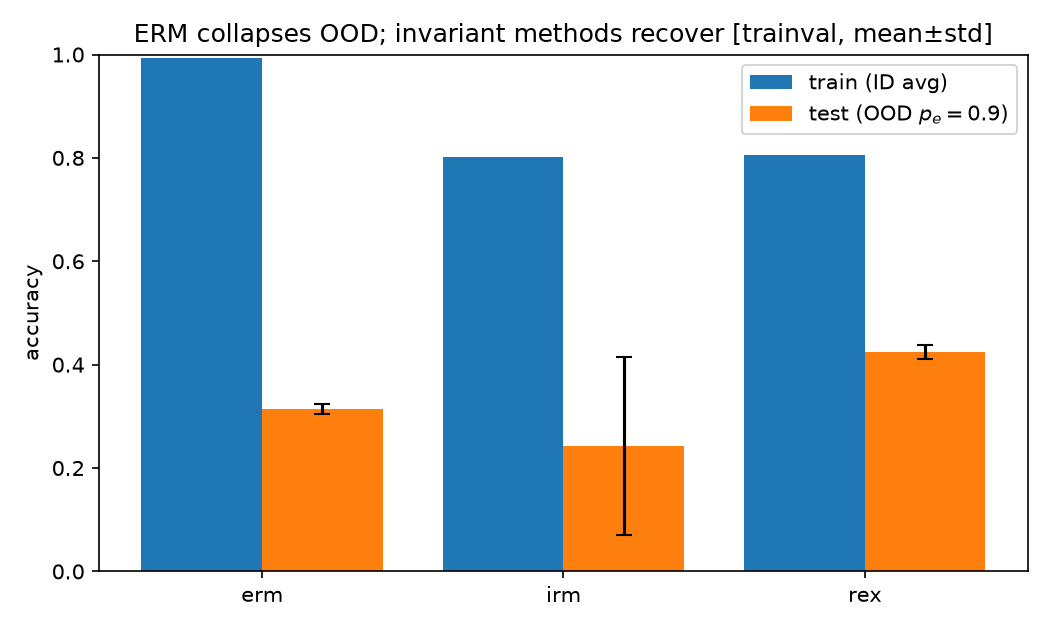
\includegraphics[width=0.8\linewidth]{figs/acc_bar.png}
\caption{Training and OOD test accuracy under train-domain validation.
Error bars indicate the standard deviation over three random seeds.}
\label{fig:accbar}
\end{figure}

\subsubsection{Effect of model selection}
The choice of model-selection protocol also affects the reported OOD performance.
Table~\ref{tab:proto} compares train-domain validation, OOD-oracle selection, and the
final checkpoint, following the distinction discussed in DomainBed
\citep{domainbed2021}.

\begin{table}[!htbp]
\centering
\small
\setlength{\tabcolsep}{4pt}
\caption{OOD accuracy under different model-selection protocols
(mean$\pm$std over 3 seeds).}
\label{tab:proto}
\begin{tabular}{lccc}
\toprule
Method & Train-domain validation & OOD oracle & Last checkpoint \\
\midrule
ERM & $0.315\pm0.010$ & $0.331\pm0.024$ & $0.304\pm0.014$ \\
IRMv1 ($\lambda=10^4$) & $0.243\pm0.172$ & $0.799\pm0.030$ & $0.754\pm0.109$ \\
V-REx ($\beta=10^3$) & $0.424\pm0.014$ & $0.563\pm0.045$ & $0.439\pm0.028$ \\
\bottomrule
\end{tabular}
\end{table}

ERM shows relatively similar OOD accuracy across the three protocols, while V-REx
shows a moderate improvement under OOD-oracle selection. IRMv1 is much more sensitive
to the selection strategy: its mean OOD accuracy increases from
$0.243\pm0.172$ under train-domain validation to $0.799\pm0.030$ under OOD-oracle
selection. The final checkpoint also reaches $0.754\pm0.109$.

These results indicate that IRMv1 can reach checkpoints with high OOD accuracy during
training, but such checkpoints are not consistently selected using only train-domain
validation. Therefore, the OOD-oracle result is used only as a reference and should
not be interpreted as a practical model-selection protocol.

\FloatBarrier
\subsection{Penalty stability (RQ2a)}

Table~\ref{tab:sweep} summarizes the penalty-strength sweep over three random
seeds. For each method and penalty strength, it reports the arithmetic mean and
sample standard deviation ($n-1$ denominator).

\begin{table}[!htbp]
\centering
\small
\setlength{\tabcolsep}{4pt}
\caption{Penalty-strength sweep under train-domain validation
(mean$\pm$std over 3 seeds).}
\label{tab:sweep}
\begin{tabular}{llccccc}
\toprule
Method & Penalty & Train & Test OOD & Gap & Worst & ECE \\
\midrule
IRMv1 & $\lambda=100$ & 0.820 & 0.365 $\pm$ 0.090 & 0.455 & 0.253 $\pm$ 0.164 & 0.137 \\
IRMv1 & $\lambda=1000$ & 0.799 & 0.286 $\pm$ 0.255 & 0.514 & 0.130 $\pm$ 0.187 & 0.399 \\
IRMv1 & $\lambda=10000$ & 0.798 & 0.286 $\pm$ 0.255 & 0.512 & 0.127 $\pm$ 0.184 & 0.404 \\
IRMv1 & $\lambda=30000$ & 0.800 & 0.281 $\pm$ 0.247 & 0.519 & 0.118 $\pm$ 0.167 & 0.407 \\
V-REx & $\beta=100$ & 0.940 & 0.293 $\pm$ 0.032 & 0.647 & 0.194 $\pm$ 0.077 & 0.064 \\
V-REx & $\beta=1000$ & 0.804 & 0.437 $\pm$ 0.033 & 0.368 & 0.343 $\pm$ 0.032 & 0.077 \\
V-REx & $\beta=10000$ & 0.785 & 0.457 $\pm$ 0.001 & 0.328 & 0.388 $\pm$ 0.021 & 0.087

\\
\bottomrule
\end{tabular}
\end{table}

Table~\ref{tab:sweep-seeds} reports the individual OOD and worst-group
accuracies underlying these averages. Each row corresponds to one method and
penalty strength; its three seed columns are separate training runs.

\begin{table}[!htbp]
\centering
\small
\setlength{\tabcolsep}{4pt}
\small
\caption{OOD and worst-group accuracy across seeds and penalty strengths.}
\label{tab:sweep-seeds}
\begin{tabular}{llccc}
\toprule
Method & Penalty & \shortstack{Seed 0\\OOD / Worst} & \shortstack{Seed 1\\OOD / Worst} & \shortstack{Seed 2\\OOD / Worst} \\
\midrule
IRMv1 & $\lambda=100$ & 0.4369 / 0.3853 & 0.3940 / 0.3029 & 0.2646 / 0.0695 \\
IRMv1 & $\lambda=1000$ & 0.1104 / 0.0000 & 0.5786 / 0.3436 & 0.1678 / 0.0449 \\
IRMv1 & $\lambda=10000$ & 0.1083 / 0.0000 & 0.5782 / 0.3383 & 0.1703 / 0.0425 \\
IRMv1 & $\lambda=30000$ & 0.1084 / 0.0000 & 0.5642 / 0.3094 & 0.1705 / 0.0443 \\
V-REx & $\beta=100$ & 0.3118 / 0.2390 & 0.3105 / 0.2383 & 0.2565 / 0.1057 \\
V-REx & $\beta=1000$ & 0.4008 / 0.3148 & 0.4643 / 0.3370 & 0.4451 / 0.3787 \\
V-REx & $\beta=10000$ & 0.4574 / 0.3975 & 0.4570 / 0.3642 & 0.4555 / 0.4022

\\
\bottomrule
\end{tabular}
\end{table}

For IRMv1, OOD accuracy changes relatively little within each seed when
$\lambda$ increases from $10^3$ to $3\times10^4$, whereas differences between
seeds are large. Over this range, seed 0 achieves OOD accuracy of approximately
$0.108$--$0.110$, seed 1 achieves $0.564$--$0.579$, and seed 2 achieves
$0.168$--$0.171$. Seed 0 has zero worst-group accuracy at all three of these
penalty strengths; seed 2 has low but nonzero worst-group accuracy
($0.042$--$0.045$). The $\lambda=10^2$ setting behaves differently, with
OOD accuracies of $0.437$, $0.394$, and $0.265$ for seeds 0, 1, and 2,
respectively. Thus, the limited sensitivity to penalty strength applies mainly
to the higher-penalty range, rather than to the entire sweep. These results
establish substantial variation between runs, but do not isolate initialization
or early training dynamics as its cause.

For V-REx, mean OOD accuracy increases from $0.293$ at $\beta=10^2$ to
$0.437$ at $\beta=10^3$ and $0.457$ at $\beta=10^4$. OOD standard deviation
does not decrease monotonically: it is $0.032$, $0.033$, and approximately
$0.001$, respectively. At $\beta=10^4$, the individual OOD accuracies are
$0.4574$, $0.4570$, and $0.4555$, showing close agreement across the tested
seeds. Worst-group accuracy remains more variable ($0.388\pm0.021$).
The highest tested V-REx penalty therefore gives more consistent OOD accuracy,
although consistency alone does not imply high predictive performance. Together,
these results support reporting both aggregate and individual-seed results.

\FloatBarrier
\subsection{Backbones, failure cases, and transfer (RQ2b)}

These experiments examine how changes to model architecture, training
environments, and data affect the behavior observed in the main Colored-MNIST
experiment. Table~\ref{tab:backbone-env} first examines backbone architecture
and the number of training environments.

\begin{table}[!htbp]
\centering
\small
\setlength{\tabcolsep}{4pt}
\caption[Backbone and environment ablations]{Backbone and environment ablations under train-domain validation
(mean$\pm$std over 3 seeds).}
\label{tab:backbone-env}
\setlength{\tabcolsep}{4pt}
\begin{tabular}{llccccc}
\toprule
Method & Configuration & Train & Test OOD & Gap & Worst & ECE \\
\midrule
ERM & MLP & 0.992 & 0.300 $\pm$ 0.006 & 0.692 & 0.219 $\pm$ 0.012 & 0.048 \\
ERM & CNN & 0.934 & 0.301 $\pm$ 0.029 & 0.633 & 0.197 $\pm$ 0.075 & 0.045 \\
IRMv1 & MLP & 0.798 & 0.286 $\pm$ 0.255 & 0.512 & 0.127 $\pm$ 0.184 & 0.404 \\
IRMv1 & CNN & 0.575 & 0.539 $\pm$ 0.084 & 0.036 & 0.099 $\pm$ 0.146 & 0.389 \\
IRMv1 & Single training environment & 0.778 & 0.431 $\pm$ 0.243 & --- & 0.211 $\pm$ 0.323 & 0.165

\\
\bottomrule
\end{tabular}
\end{table}

\subsubsection{Backbone architecture}
Table~\ref{tab:backbone-env} compares the MLP used in the main experiments with a small CNN. Under
train-domain validation, the CNN achieves an OOD accuracy of
$0.539\pm0.084$, compared with $0.286\pm0.255$ for the MLP. The CNN therefore shows
both a higher mean OOD accuracy and lower variation in this experiment.

However, its worst-group accuracy remains relatively low, indicating that improved
average OOD accuracy does not necessarily correspond to uniformly good performance
across all label--color groups. The backbone architecture therefore affects the
observed performance, but does not by itself remove the difficulties caused by the
spurious correlation.

\subsubsection{Single training environment}
Table~\ref{tab:backbone-env} also reports IRMv1 with only one training environment. The resulting
OOD accuracy is $0.431\pm0.243$, with a large standard deviation across the three
random seeds. Although the mean accuracy is not uniformly low, the large variation
indicates that the result is considerably less stable when the model cannot compare
patterns across multiple environments. This setting removes an important source of
information used by invariant learning: variation between environments.

Table~\ref{tab:robust-transfer} examines additional spurious features,
reduced sample size, and transfer to Colored-FashionMNIST.

\begin{table}[!htbp]
\centering
\small
\setlength{\tabcolsep}{4pt}
\caption[Spurious features, sample size, and dataset transfer]{Spurious-feature, sample-size, and dataset-transfer ablations under train-domain validation
(mean$\pm$std over 3 seeds).}
\label{tab:robust-transfer}
\setlength{\tabcolsep}{4pt}
\begin{tabular}{llccccc}
\toprule
Method & Configuration & Train & Test OOD & Gap & Worst & ECE \\
\midrule
ERM & Additional $3\times3$ patch & 0.998 & 0.146 $\pm$ 0.002 & 0.853 & 0.089 $\pm$ 0.005 & 0.020 \\
IRMv1 & Additional $3\times3$ patch & 0.909 & 0.117 $\pm$ 0.008 & 0.791 & 0.080 $\pm$ 0.026 & 0.325 \\
ERM & $n=6{,}250$ per environment & 1.000 & 0.289 $\pm$ 0.003 & 0.711 & 0.212 $\pm$ 0.005 & 0.012 \\
IRMv1 & $n=6{,}250$ per environment & 0.756 & 0.356 $\pm$ 0.272 & 0.400 & 0.119 $\pm$ 0.138 & 0.306 \\
ERM & Colored-FashionMNIST & 0.944 & 0.260 $\pm$ 0.009 & 0.684 & 0.161 $\pm$ 0.021 & 0.178 \\
IRMv1 & Colored-FashionMNIST & 0.600 & 0.650 $\pm$ 0.063 & -0.050 & 0.346 $\pm$ 0.148 & 0.218

\\
\bottomrule
\end{tabular}
\end{table}

\subsubsection{Additional spurious feature}
We introduce a second spurious feature in the form of a $3\times3$ patch
(Table~\ref{tab:robust-transfer}).
Under this setting, the OOD accuracy of IRMv1 decreases to
$0.117\pm0.008$, which is close to the ERM result of $0.146\pm0.002$.
This result is consistent with the theoretical analysis of
\citet{rosenfeld2021risks}, which relates the ability to identify invariant features
to the number of environments relative to the number of independent spurious
features. In this experiment, adding another spurious signal makes the invariant
learning problem more difficult without adding another training environment.

\subsubsection{Limited training data}
The small-$n$ setting in Table~\ref{tab:robust-transfer} reduces each training
environment to 6,250 samples. Compared
with the standard setting, the results show greater variation across random seeds.
This suggests that reducing the amount of training data can make the learned solution
less stable. Since both the stable digit-shape signal and the spurious color signal
must be estimated from fewer observations, differences caused by initialization and
optimization may have a larger effect on the final model.

\subsubsection{Transfer to Colored-FashionMNIST}
Finally, we repeat the same environment-generation procedure using FashionMNIST
instead of MNIST. Under this setting, IRMv1 achieves an OOD accuracy of
$0.650\pm0.063$, while ERM obtains $0.260\pm0.009$. This shows that the difference
between ERM and IRMv1 observed in Colored-MNIST is not limited to the original MNIST
digits under the tested transfer setting.

Overall, these experiments show that the behavior of invariant learning depends on
several properties of the experimental setting. Additional spurious features, fewer
environments, and reduced training data can make the problem less stable, while the
choice of backbone can substantially change the observed OOD accuracy. The
Colored-FashionMNIST experiment further provides a second dataset on which the same
evaluation procedure can be examined.

\FloatBarrier
\subsection{Diagnostics (RQ3)}

The previous experiments evaluate the models mainly through predictive performance.
To better understand how the models use the available information, we also examine
their calibration, input attributions, and learned representations.

\subsubsection{Calibration}
Figure~\ref{fig:rel} compares the reliability diagrams of ERM and IRM on the OOD test
set. ERM obtains an ECE of $0.055$, while IRM obtains a higher ECE of $0.231$.
This indicates that the two models differ not only in OOD accuracy but also in how
well their predicted confidence matches the observed correctness.

\begin{figure}[!htbp]
\centering
\begin{subfigure}{0.38\linewidth}
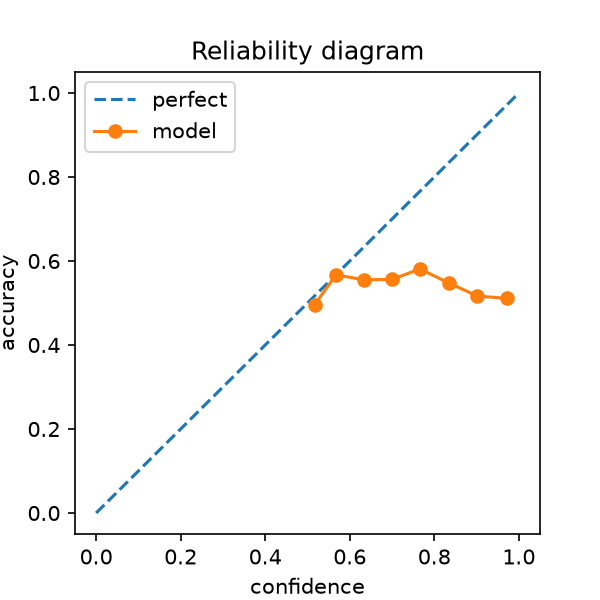
\includegraphics[width=\linewidth]{figs/reliability_erm.png}
\caption{ERM (OOD, ECE $0.055$).}
\end{subfigure}\hspace{0.06\linewidth}
\begin{subfigure}{0.38\linewidth}
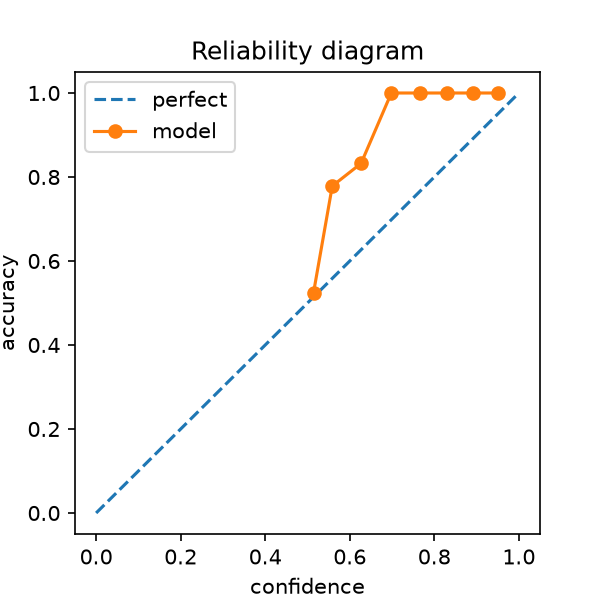
\includegraphics[width=\linewidth]{figs/reliability_irm.png}
\caption{IRM (OOD, ECE $0.231$).}
\end{subfigure}
\caption{Reliability diagrams on the OOD test set. The diagonal represents perfect calibration.}
\label{fig:rel}
\end{figure}

\subsubsection{Attribution analysis}
To inspect which parts of the input contribute to the prediction, we use Integrated
Gradients as the main attribution method. Figure~\ref{fig:ig} shows that the
attributions of ERM are more strongly associated with the color-related regions,
while IRM places relatively more emphasis on the digit strokes.

\begin{figure}[H]
\centering
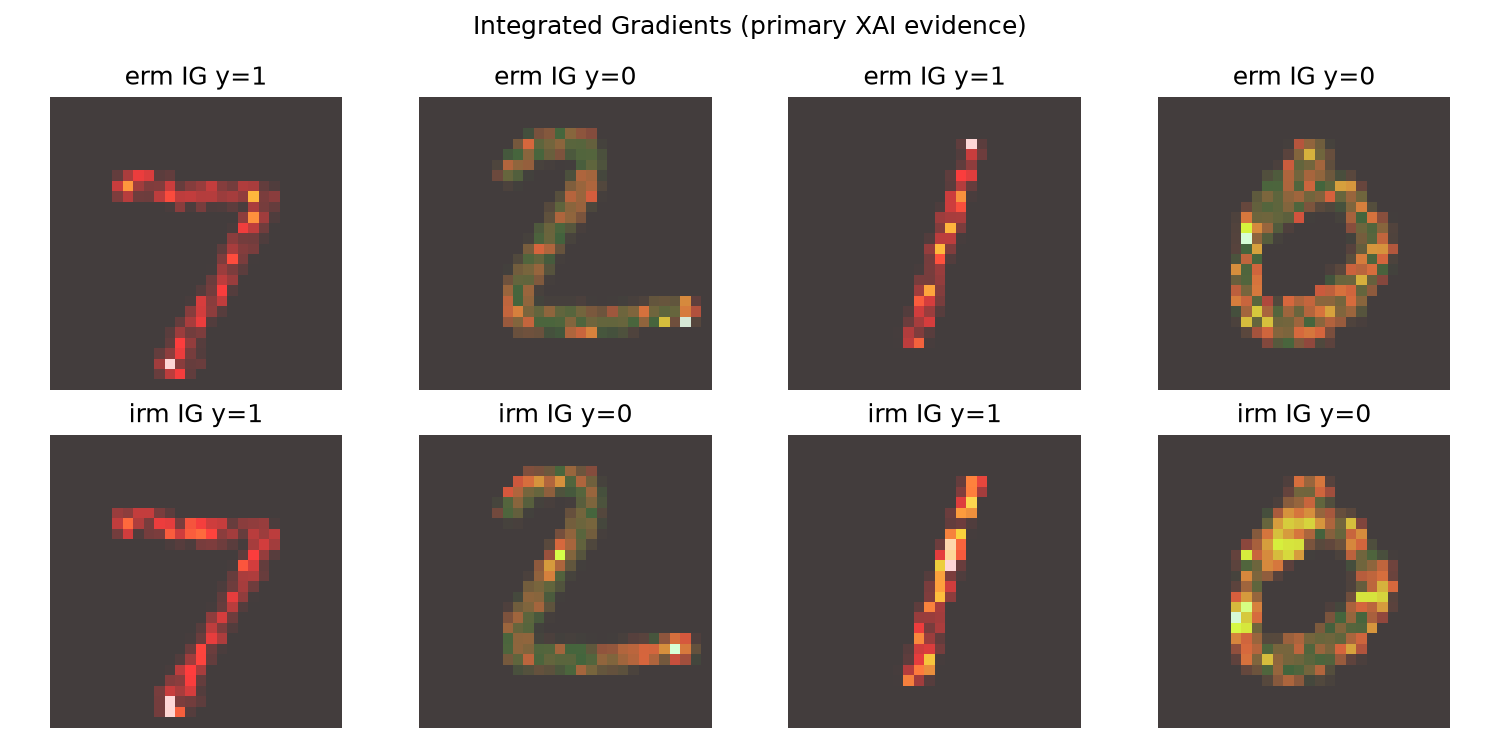
\includegraphics[width=0.70\linewidth]{figs/ig_erm_vs_irm.png}
\caption{Integrated Gradients for ERM (top row) and IRM (bottom row). ERM shows stronger
attribution to color-related regions, while IRM places more emphasis on digit strokes.}
\label{fig:ig}
\end{figure}

For reference, we also report vanilla saliency maps in Fig.~\ref{fig:sal}. However,
vanilla saliency is used only as a secondary baseline because gradient-based saliency
methods are known to fail several sanity checks \citep{adebayo2018sanity}.

\begin{figure}[!htbp]
\centering
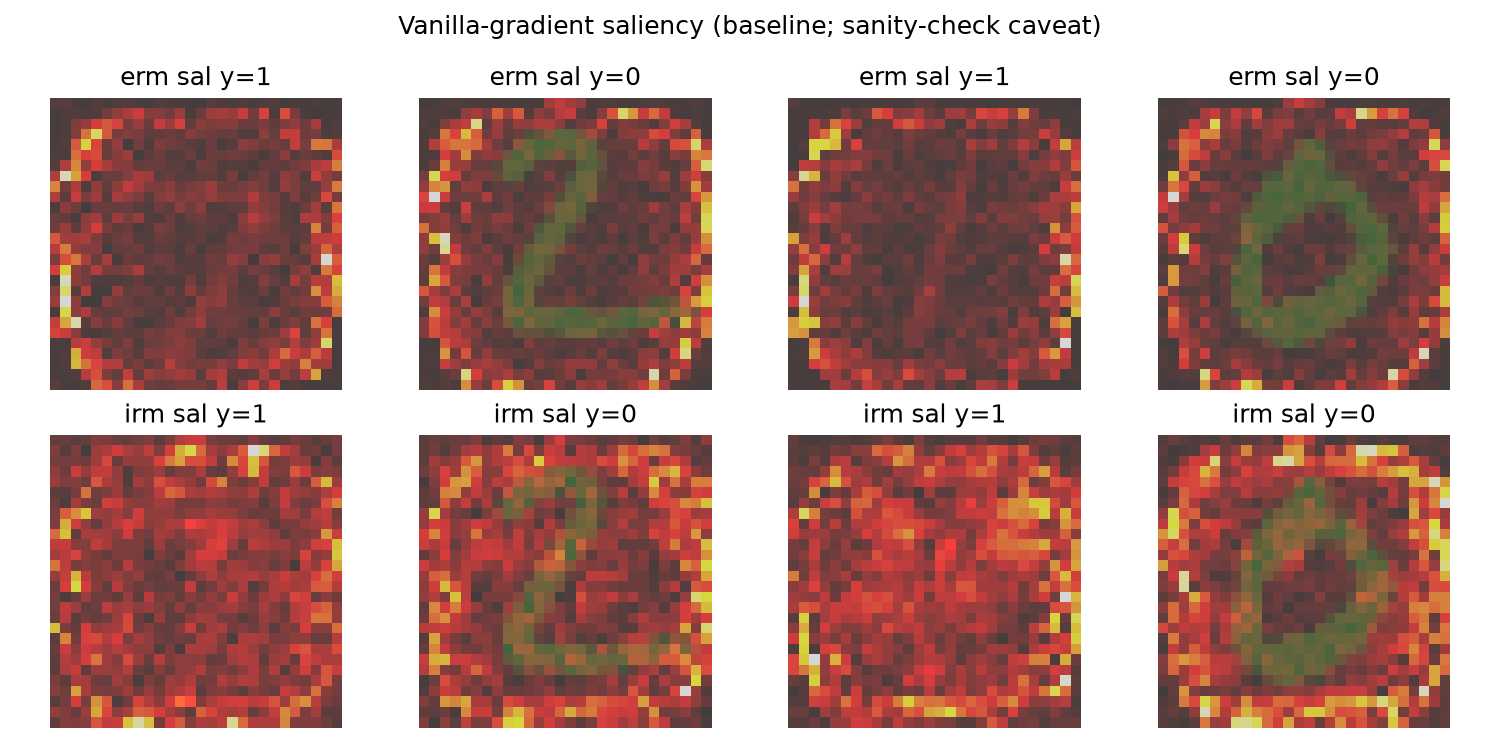
\includegraphics[width=0.72\linewidth]{figs/saliency_erm_vs_irm.png}
\caption{Vanilla saliency maps for ERM and IRM. These results are included as a
secondary baseline; Integrated Gradients in Fig.~\ref{fig:ig} is used as the main
attribution analysis.}
\label{fig:sal}
\end{figure}

\subsubsection{Representation probe}
Finally, we train a linear probe on the penultimate-layer representations to predict
the color variable. The probe reaches a held-out accuracy of $1.00$ for both ERM and
IRM, showing that color information remains fully decodable from the learned
representations in both cases.

This result is important when interpreting the attribution results. Although IRM
appears to rely less on color for its final prediction, the color information has not
been removed from the representation itself. Instead, the difference may occur in how
the final classification layer uses the available features. This observation is
consistent with previous findings that useful and spurious information can remain in
the learned representation while being weighted differently by the final classifier
\citep{kirichenko2022dfr}.

% ============================================================
% ============================================================
% PART 6 — CONCLUSION
% ============================================================
\clearpage
\section{Conclusion}
\label{sec:conclusion}

This report examined how spurious correlations affect out-of-distribution
(OOD) generalization on Colored-MNIST. ERM, IRMv1, and V-REx were compared
using a common pipeline, three random seeds, and complementary diagnostics.

For \textbf{RQ1}, high training accuracy did not translate into reliable OOD
performance. ERM achieved an OOD accuracy of $0.315\pm0.010$. IRMv1 was
particularly sensitive to checkpoint selection: its accuracy increased from
$0.243\pm0.172$ under train-domain selection to $0.799\pm0.030$ under
OOD-oracle selection. This difference shows that reaching a useful checkpoint
and selecting it without OOD information are separate challenges. The oracle
result is therefore a diagnostic reference rather than a practical selection rule.

For \textbf{RQ2}, increasing the IRMv1 penalty did not consistently improve
performance. Results varied substantially between seeds, while changing
$\lambda$ within the higher-penalty range had relatively little effect within
each seed. V-REx attained its most consistent OOD result at $\beta=10^4$
($0.457\pm0.001$), although low variance alone does not imply high accuracy.
Backbone architecture, the number of environments, an additional spurious
patch, and sample size also affected performance. Colored-FashionMNIST
provided a second dataset for testing the same evaluation procedure.

For \textbf{RQ3}, attribution and probe analyses distinguished the information
encoded in a representation from the information used for prediction.
Integrated Gradients suggested greater attention to digit shape for IRM than
for ERM, yet a linear color probe achieved held-out accuracy of $1.00$ for
both models. Reduced apparent reliance on color therefore did not imply that
color information had been removed from the representation.

These findings support reporting checkpoint-selection rules, individual-seed
results, and diagnostics alongside average OOD accuracy. Penalty strength
should be assessed together with architecture and training conditions rather
than treated as a sufficient guarantee of invariance.

The conclusions are limited to the tested synthetic shifts in MNIST and
FashionMNIST. Real-world datasets such as Waterbirds or CelebA, larger models,
and broader hyperparameter searches remain directions for future work.
The present results characterize the evaluated settings and do not establish
a general ranking of OOD learning methods.

\clearpage
% REFERENCES: add or update entries in references.bib.
\phantomsection
\addcontentsline{toc}{section}{References}
\markboth{References}{}
\bibliographystyle{unsrtnat}
\bibliography{references}

\appendix
\clearpage
\section{Reproducibility}
\setstretch{1}
\setlength{\parskip}{2pt}
\titlespacing*{\subsection}{0pt}{8pt}{4pt}
\RecustomVerbatimEnvironment{verbatim}{Verbatim}{fontsize=\footnotesize,baselinestretch=0.95}
\setlength{\parskip}{0pt}
\setlist{topsep=2pt,itemsep=1pt,parsep=0pt}

The source code, experiment configurations, and scripts used in this report are
available at:

\begin{center}
\url{https://github.com/namng194/spurious-correlations-invariant-learning}
\end{center}

\subsection{Environment setup}
The experiments were run with Python 3.12. The environment can be created using:

\begin{verbatim}
uv venv --python 3.12 .venv
uv sync --extra dev
\end{verbatim}

The test suite can be executed with:

\begin{verbatim}
.venv/bin/python -m pytest tests/ -x -q
\end{verbatim}

\subsection{Main experiments}
The main experiments can be reproduced with:

\begin{verbatim}
.venv/bin/python scripts/run_sweep.py \
  --config configs/base.yaml \
  --out outputs/sweep
\end{verbatim}

The extended ablation experiments can be reproduced with:

\begin{verbatim}
.venv/bin/python scripts/ablate.py \
  --config configs/heavy.yaml \
  --out outputs/ablate
\end{verbatim}

\subsection{Figures and diagnostics}
The main plots are generated with:

\begin{verbatim}
.venv/bin/python scripts/make_plots.py \
  --in outputs/sweep/results.json \
  --out outputs/figs
\end{verbatim}

Diagnostic figures are generated with:

\begin{verbatim}
.venv/bin/python scripts/make_diagnostics.py \
  --config configs/fast.yaml \
  --out outputs/figs
\end{verbatim}

\Needspace{6\baselineskip}
\subsection{Saved results}
The raw experimental results are stored in:

\begin{itemize}
    \item \texttt{outputs/sweep/results.json}
    \item \texttt{outputs/ablate/ablate\_full.json}
\end{itemize}

These files contain the values used to generate the tables and figures reported in
Section~\ref{sec:results}.


\end{document}
